%%%%%%%%%%%%%%%%%%%%%%%%%%%%%%%%%%%%%%%%%%%%%%%%%%%
\begin{frame}
  \begin{center}
    {\Large CNN using PyTorch}
    
  \end{center}
  
  % \tiny{(Ref: PyTorch Zero To All Lecture by Sung Kim)}
\end{frame}

%%%%%%%%%%%%%%%%%%%%%%%%%%%%%%%%%%%%%%%%%%%%%%%%%%%
\begin{frame}[fragile] \frametitle{Image Processing Algorithms}

In Computer Vision, following are some of the popular usecases:

\begin{itemize}
\item Image Classification is the simplest task, when we need to classify an image into one of many pre-defined categories, for example, distinguish a cat from a dog on a photograph, or recognize a handwritten digit.

\item Object Detection is a bit more difficult task, in which we need to find known objects on the picture and localize them, i.e. return the bounding box for each of recognized objects.

\item Segmentation is similar to object detection, but instead of giving bounding box we need to return an exact pixel map outlining each of the recognized objects.
\end{itemize}

\begin{center}
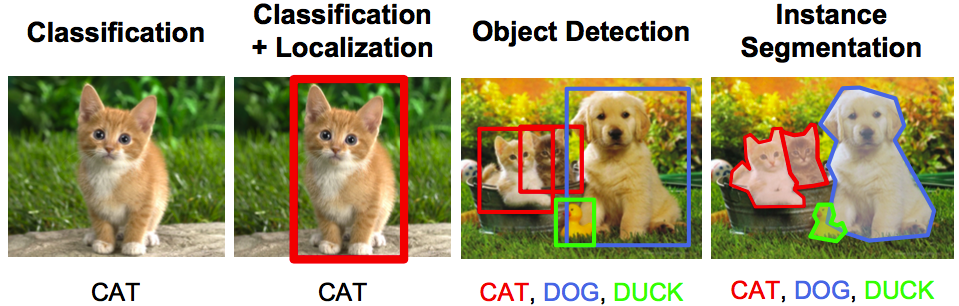
\includegraphics[width=0.9\linewidth,keepaspectratio]{pyt41}
\end{center}

\tiny{(Ref: Microsoft - Intro to Machine Learning using Pytorch)}
\end{frame}

%%%%%%%%%%%%%%%%%%%%%%%%%%%%%%%%%%%%%%%%%%%%%%%%%%%
\begin{frame}[fragile] \frametitle{Images as Tensors}


\begin{itemize}
\item Images consist of pixels, so they can be thought of as a rectangular collection (array) of pixels.
\item Each pixel is actually a number either in the scale of range 0 to 1 (in which case floating point numbers are used), or 0 to 255 (integers), for gray scale.
\item For color images, each pixel has 3 values (called channels) RGB, and thus color image of size  $W×H$  will be represented as an array of size $3×H×W$
  (sometimes the order of components might be different, but the idea is the same).
	\item Multi-dimensional arrays are also called tensors. 
	\item Using tensors to represent images also has an advantage, because we can use an extra dimension to store a sequence of images.
	\item For example, to represent a video fragment consisting of $200$ frames with $800x600$ dimension, we may use the tensor of size $200x3x600x800$.
\end{itemize}


\tiny{(Ref: Microsoft - Intro to Machine Learning using Pytorch)}
\end{frame}


%%%%%%%%%%%%%%%%%%%%%%%%%%%%%%%%%%%%%%%%%%%%%%%%%%%
\begin{frame}[fragile] \frametitle{Import MNIST}

\lstinline|torchvison.datasets.MNIST| is  in the form of Python Imagine Library (PIL) images, which we convert to tensors by passing a \lstinline|transform=ToTensor()| parameter.

\begin{lstlisting}
from torchvision.transforms import ToTensor

data_train = torchvision.datasets.MNIST('./data',
        download=True,train=True,transform=ToTensor())
data_test = torchvision.datasets.MNIST('./data',
        download=True,train=False,transform=ToTensor())
\end{lstlisting}

Dataset has  a total of 6000 training images and 1000 testing images. Each sample is a tuple with the first element is a tensor of 1x28x28 size and the second  element is a label that specifies which digit is represented by the tensor

\begin{lstlisting}
print('Training samples:',len(data_train))
print('Test samples:',len(data_test))

print('Tensor size:',data_train[0][0].size())
print('First 10 digits are:', [data_train[i][1] for i in range(10)])

>>>Training samples: 60000
Test samples: 10000
Tensor size: torch.Size([1, 28, 28])
First 10 digits are: [5, 0, 4, 1, 9, 2, 1, 3, 1, 4]
\end{lstlisting}



\tiny{(Ref: Microsoft - Intro to Machine Learning using Pytorch)}
\end{frame}

%%%%%%%%%%%%%%%%%%%%%%%%%%%%%%%%%%%%%%%%%%%%%%%%%%%
\begin{frame}[fragile] \frametitle{Visualize MNIST}


\begin{lstlisting}
fig,ax = plt.subplots(1,7)
for i in range(7):
    ax[i].imshow(data_train[i][0].view(28,28))
    ax[i].set_title(data_train[i][1])
    ax[i].axis('off')
\end{lstlisting}

\begin{center}
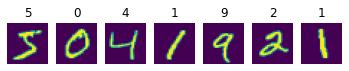
\includegraphics[width=0.9\linewidth,keepaspectratio]{pyt42}
\end{center}


\tiny{(Ref: Microsoft - Intro to Machine Learning using Pytorch)}
\end{frame}


%%%%%%%%%%%%%%%%%%%%%%%%%%%%%%%%%%%%%%%%%%%%%%%%%%%
\begin{frame}[fragile] \frametitle{Training a dense neural network, NOT concolutional}

The simplest network would include just one fully-connected layer, which is called Linear layer, with 784 inputs (one input for each pixel of the input image) and 10 outputs (one output for each class).

\begin{center}
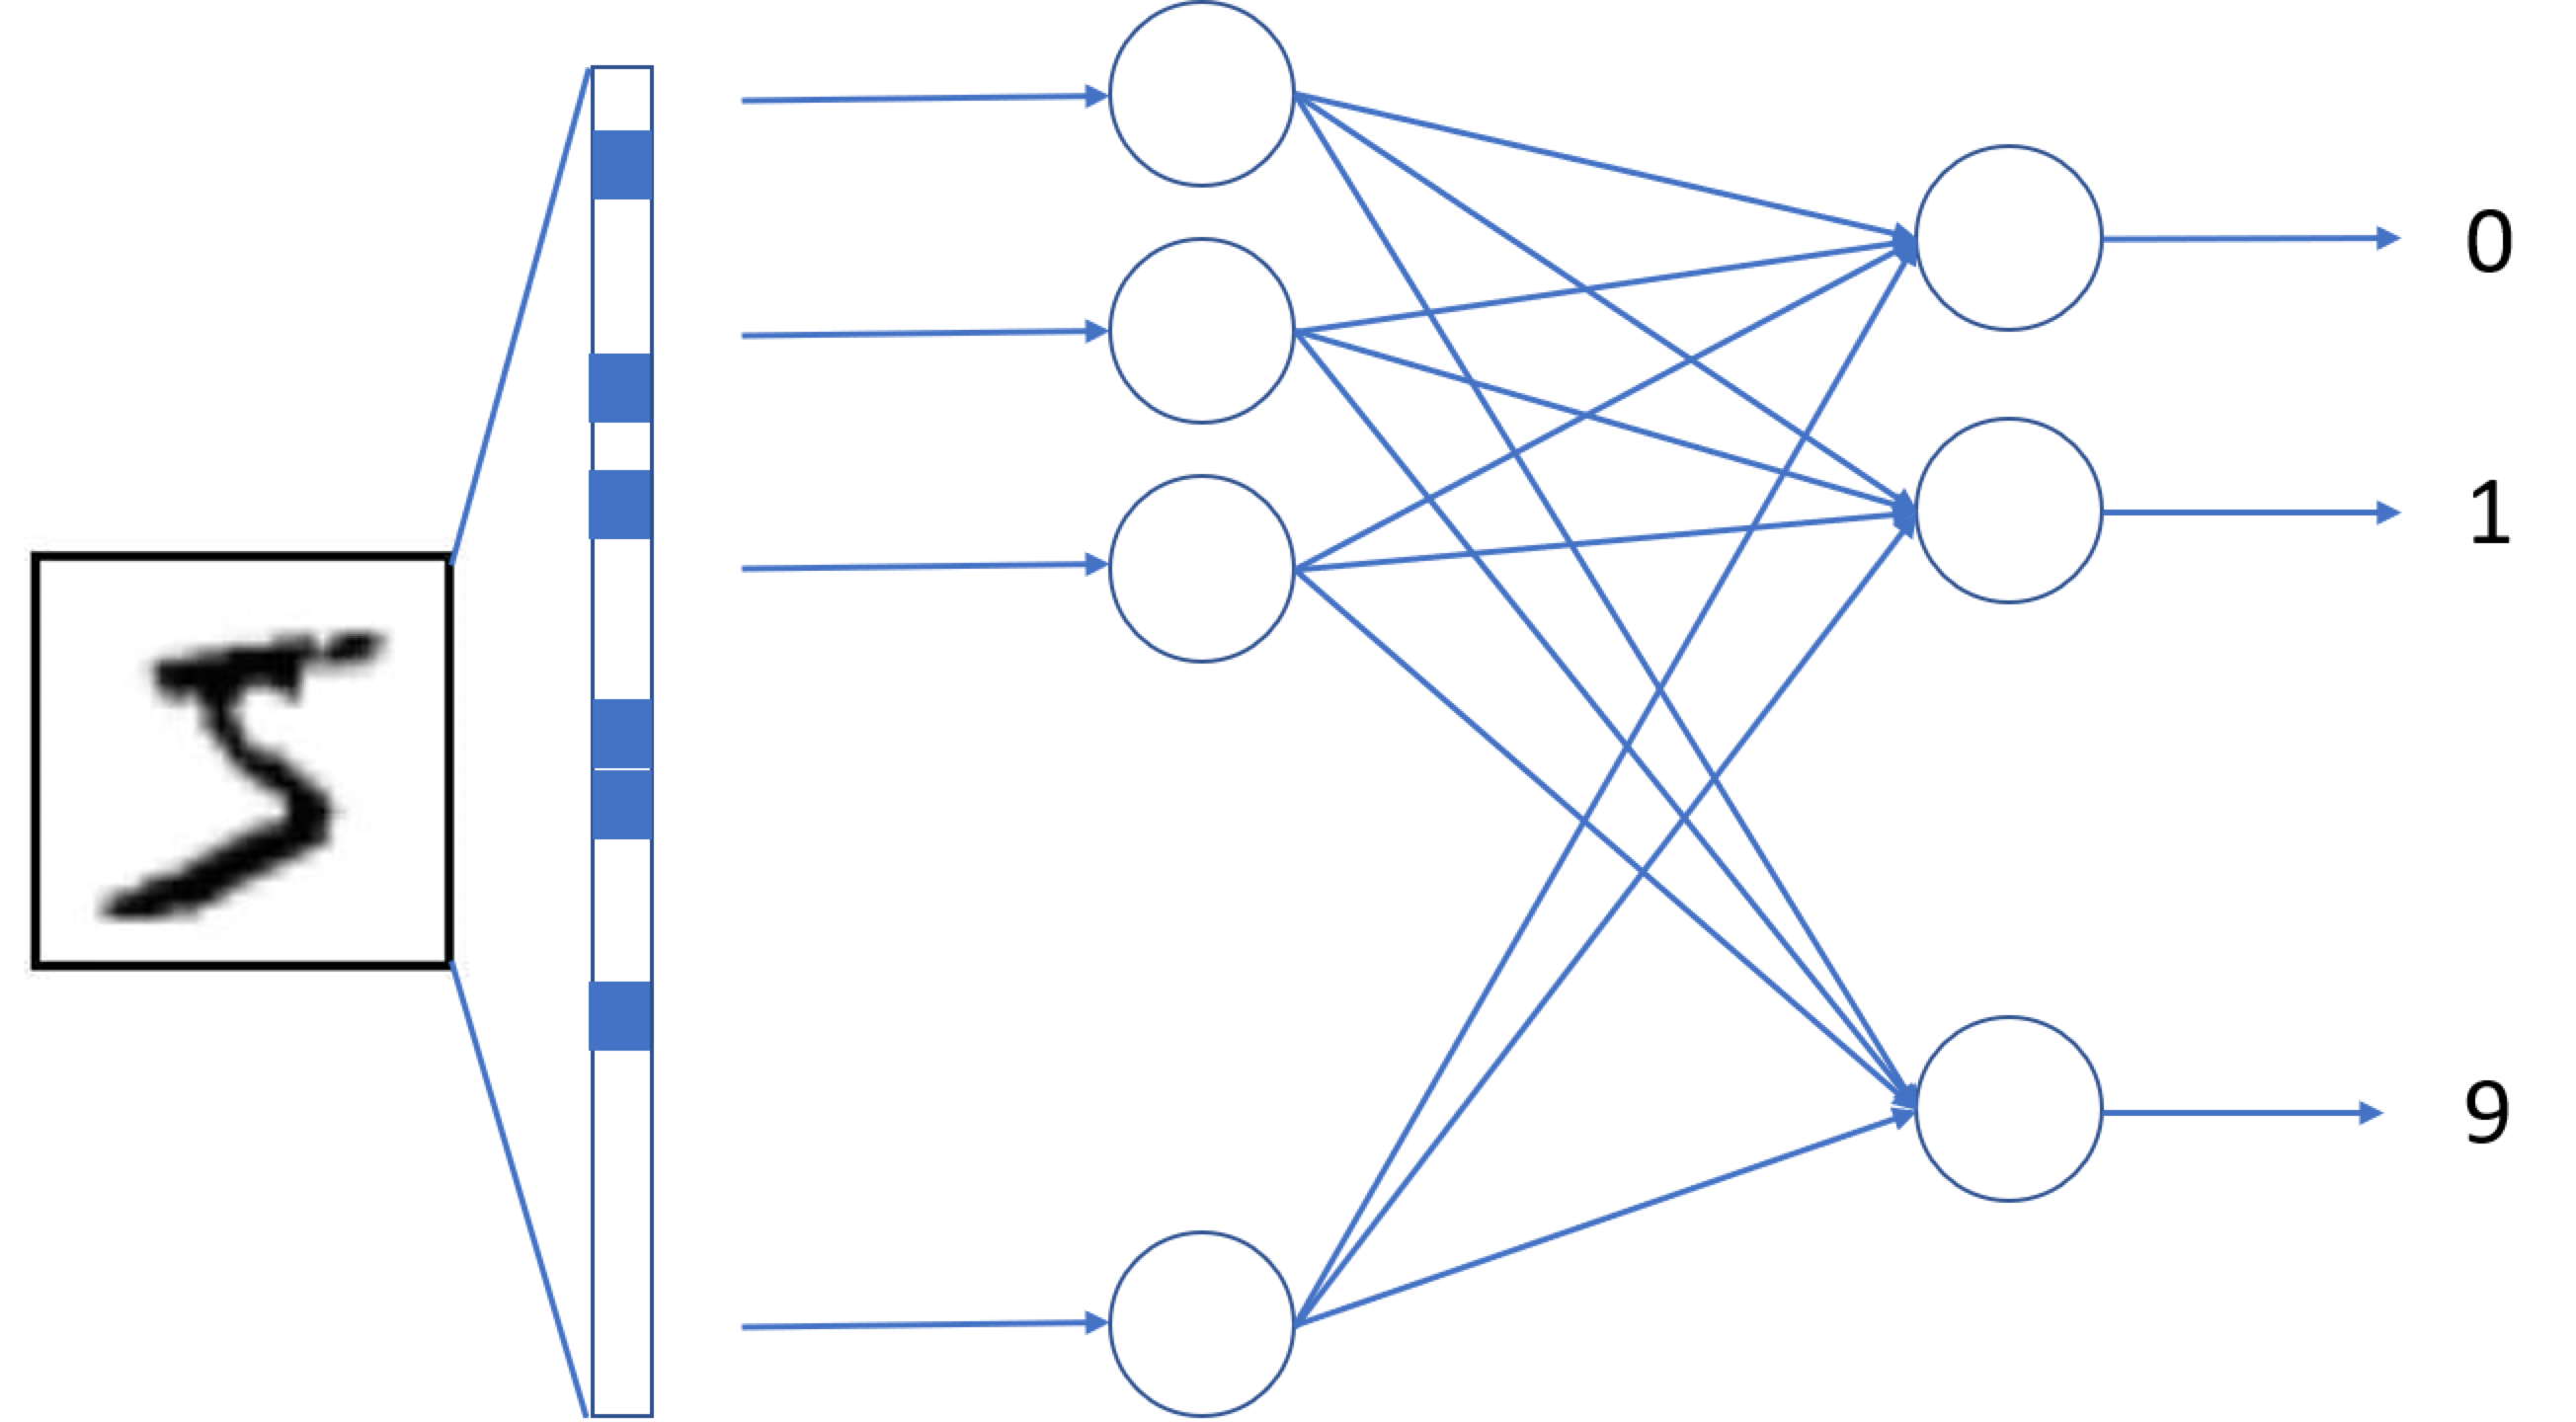
\includegraphics[width=0.9\linewidth,keepaspectratio]{pyt43}

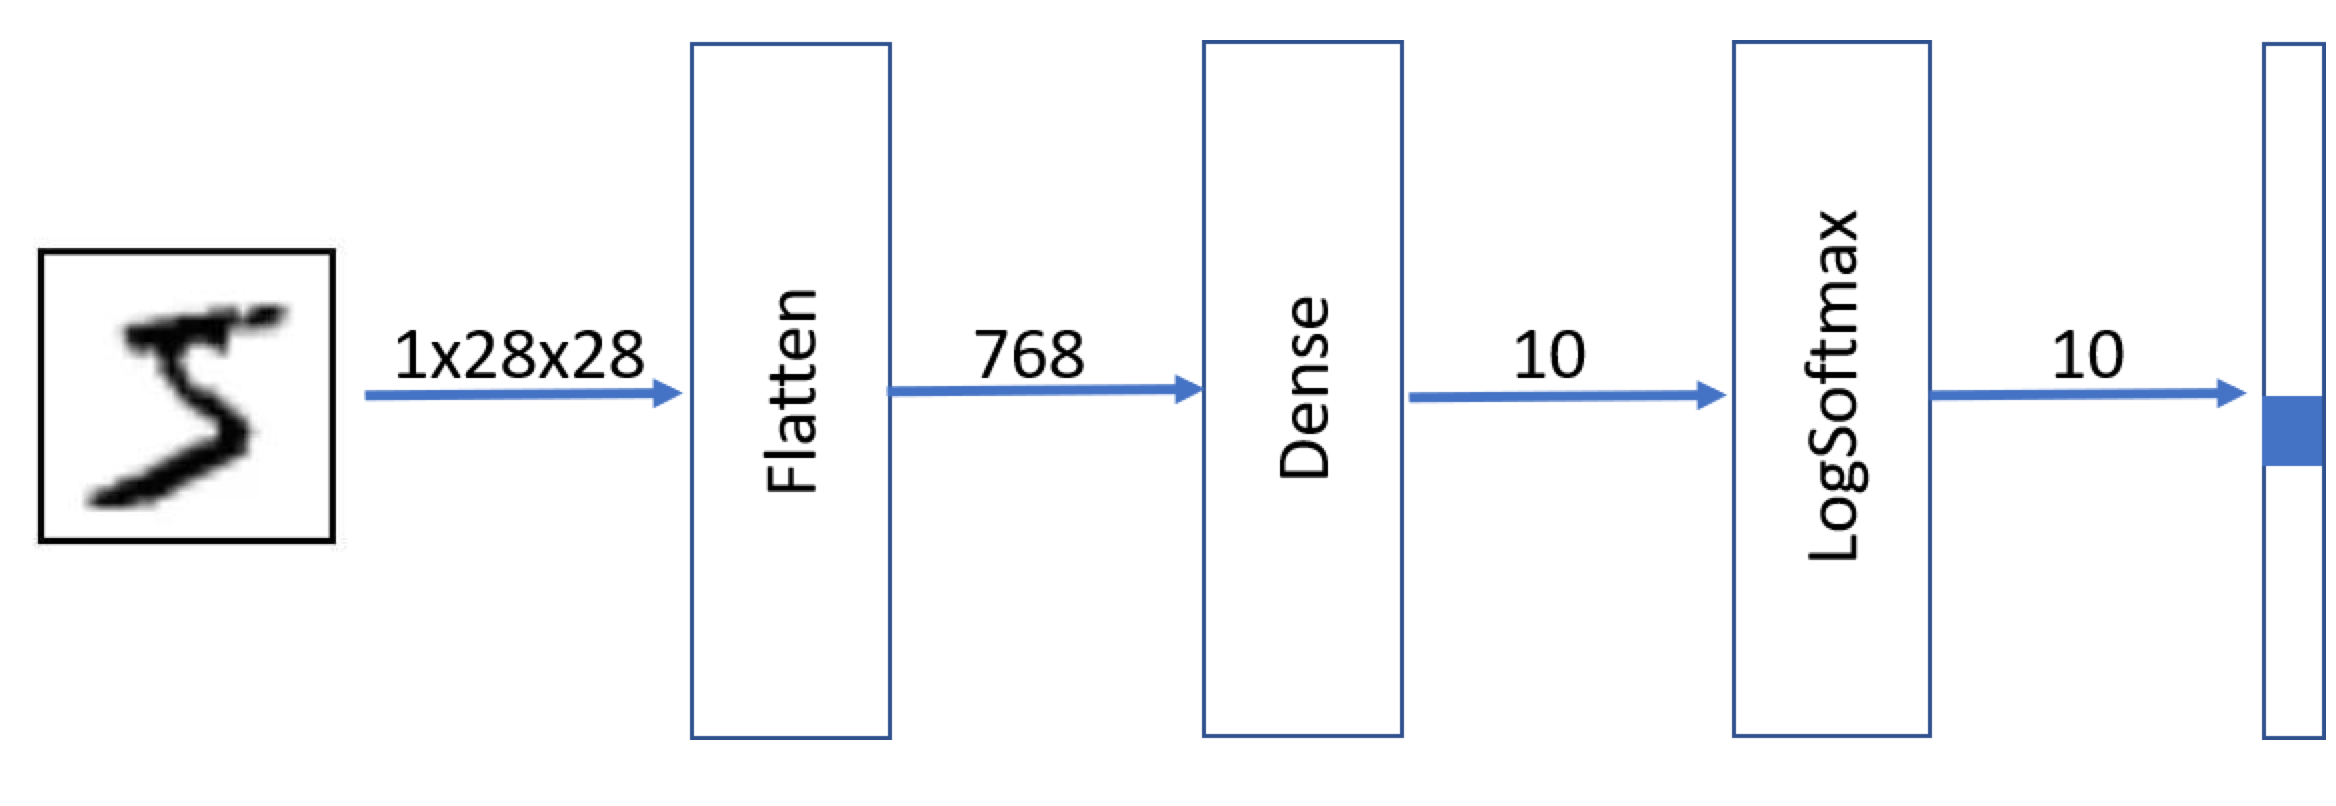
\includegraphics[width=0.9\linewidth,keepaspectratio]{pyt44}

\end{center}



\begin{lstlisting}
net = nn.Sequential(
        nn.Flatten(), 
        nn.Linear(784,10), # 784 inputs, 10 outputs
        nn.LogSoftmax())
\end{lstlisting}

\tiny{(Ref: Microsoft - Intro to Machine Learning using Pytorch)}
\end{frame}

%%%%%%%%%%%%%%%%%%%%%%%%%%%%%%%%%%%%%%%%%%%%%%%%%%%
\begin{frame}[fragile] \frametitle{Training a dense neural network, NOT concolutional}


Given any digit as input and produce a vector of probabilities as an output.


\begin{lstlisting}
print('Digit to be predicted: ',data_train[0][1])
torch.exp(net(data_train[0][0]))

>>>tensor([[0.0977, 0.0959, 0.1033, 0.1033, 0.0824, 0.1087, 0.0955, 0.0895, 0.1338,
         0.0900]], grad_fn=<ExpBackward>)
\end{lstlisting}

As you can see the network predicts similar probabilities for each digit. This is because it has not been trained on how to recognize the digits. We need to give it our training data to train it on our dataset.

\tiny{(Ref: Microsoft - Intro to Machine Learning using Pytorch)}
\end{frame}

%%%%%%%%%%%%%%%%%%%%%%%%%%%%%%%%%%%%%%%%%%%%%%%%%%%
\begin{frame}[fragile] \frametitle{Training a dense neural network, NOT concolutional}


To train the model we will need to create batches of our datasets of a certain size, let's say 64. PyTorch has an object called DataLoader that can create batches of our data for us automatically:

\begin{lstlisting}
train_loader = torch.utils.data.DataLoader(data_train,batch_size=64)
test_loader = torch.utils.data.DataLoader(data_test,batch_size=64) # we can use larger batch size for testing
\end{lstlisting}



\tiny{(Ref: Microsoft - Intro to Machine Learning using Pytorch)}
\end{frame}

%%%%%%%%%%%%%%%%%%%%%%%%%%%%%%%%%%%%%%%%%%%%%%%%%%%
\begin{frame}[fragile] \frametitle{Training a dense neural network, NOT concolutional}

Training Steps:

\begin{itemize}
\item We take a minibatch from the input dataset, which consists of input data (features) and expected result (label).
\item We calculate the predicted result for this minibatch.
The difference between this result and expected result is calculated using a special function called the loss function
\item We calculate the gradients of this loss function with respect to model weights (parameters), which are then used to adjust the weights to optimize the performance of the network. The amount of adjustment is controlled by a parameter called learning rate, and the details of optimization algorithm are defined in the optimizer object.
\item We repeat those steps until the whole dataset is processed. One complete pass through the dataset is called an epoch.
\end{itemize}


\tiny{(Ref: Microsoft - Intro to Machine Learning using Pytorch)}
\end{frame}


%%%%%%%%%%%%%%%%%%%%%%%%%%%%%%%%%%%%%%%%%%%%%%%%%%%
\begin{frame}[fragile] \frametitle{Training a dense neural network, NOT concolutional}

Build a generic training function that takes the following parameters:

\begin{itemize}
\item Neural network
\item DataLoader, which defines the data to train on
\item Loss Function, for classification tasks NLLLoss is used
\item Optimizer, Adam by default.
\item Learning rate 
\end{itemize}

\begin{lstlisting}
def train_epoch(net,dataloader,lr=0.01,optimizer=None,loss_fn = nn.NLLLoss()):
    optimizer = optimizer or torch.optim.Adam(net.parameters(),lr=lr)
    net.train()
    total_loss,acc,count = 0,0,0
    for features,labels in dataloader:
        optimizer.zero_grad()
        out = net(features)
        loss = loss_fn(out,labels) #cross_entropy(out,labels)
        loss.backward()
        optimizer.step()
        total_loss+=loss
        _,predicted = torch.max(out,1)
        acc+=(predicted==labels).sum()
        count+=len(labels)
    return total_loss.item()/count, acc.item()/count

train_epoch(net,train_loader)

>>> (0.00593234608968099, 0.8924166666666666)

\end{lstlisting}


\tiny{(Ref: Microsoft - Intro to Machine Learning using Pytorch)}
\end{frame}

%%%%%%%%%%%%%%%%%%%%%%%%%%%%%%%%%%%%%%%%%%%%%%%%%%%
\begin{frame}[fragile] \frametitle{Training a dense neural network, NOT concolutional}

Similarly, build a generic validation function 

\begin{lstlisting}
def validate(net, dataloader,loss_fn=nn.NLLLoss()):
    net.eval()
    count,acc,loss = 0,0,0
    with torch.no_grad():
        for features,labels in dataloader:
            out = net(features)
            loss += loss_fn(out,labels) 
            pred = torch.max(out,1)[1]
            acc += (pred==labels).sum()
            count += len(labels)
    return loss.item()/count, acc.item()/count

validate(net,test_loader)

>>> (0.00586661148071289, 0.8935)
\end{lstlisting}


\tiny{(Ref: Microsoft - Intro to Machine Learning using Pytorch)}
\end{frame}

%%%%%%%%%%%%%%%%%%%%%%%%%%%%%%%%%%%%%%%%%%%%%%%%%%%
\begin{frame}[fragile] \frametitle{Training a dense neural network, NOT concolutional}

Combo generic function

\begin{lstlisting}
def train(net,train_loader,test_loader,optimizer=None,lr=0.01,epochs=10,loss_fn=nn.NLLLoss()):
    optimizer = optimizer or torch.optim.Adam(net.parameters(),lr=lr)
    res = { 'train_loss' : [], 'train_acc': [], 'val_loss': [], 'val_acc': []}
    for ep in range(epochs):
        tl,ta = train_epoch(net,train_loader,optimizer=optimizer,lr=lr,loss_fn=loss_fn)
        vl,va = validate(net,test_loader,loss_fn=loss_fn)
        print(f"Epoch {ep:2}, Train acc={ta:.3f}, Val acc={va:.3f}, Train loss={tl:.3f}, Val loss={vl:.3f}")
        res['train_loss'].append(tl)
        res['train_acc'].append(ta)
        res['val_loss'].append(vl)
        res['val_acc'].append(va)
    return res

# Re-initialize the network to start from scratch
net = nn.Sequential(
        nn.Flatten(), 
        nn.Linear(784,10), # 784 inputs, 10 outputs
        nn.LogSoftmax())

hist = train(net,train_loader,test_loader,epochs=5)		
\end{lstlisting}


\tiny{(Ref: Microsoft - Intro to Machine Learning using Pytorch)}
\end{frame}

%%%%%%%%%%%%%%%%%%%%%%%%%%%%%%%%%%%%%%%%%%%%%%%%%%%
\begin{frame}[fragile] \frametitle{Training a dense neural network, NOT concolutional}

Training function logs messages with the accuracy on training and validation data from each epoch. It also returns this data as a dictionary (called history). We can then visualize this data to better understand our model training.

\begin{lstlisting}
plt.figure(figsize=(15,5))
plt.subplot(121)
plt.plot(hist['train_acc'], label='Training acc')
plt.plot(hist['val_acc'], label='Validation acc')
plt.legend()
plt.subplot(122)
plt.plot(hist['train_loss'], label='Training loss')
plt.plot(hist['val_loss'], label='Validation loss')
plt.legend()
\end{lstlisting}


\tiny{(Ref: Microsoft - Intro to Machine Learning using Pytorch)}
\end{frame}


%%%%%%%%%%%%%%%%%%%%%%%%%%%%%%%%%%%%%%%%%%%%%%%%%%%
\begin{frame}[fragile] \frametitle{Training a dense neural network, NOT concolutional}

\begin{center}
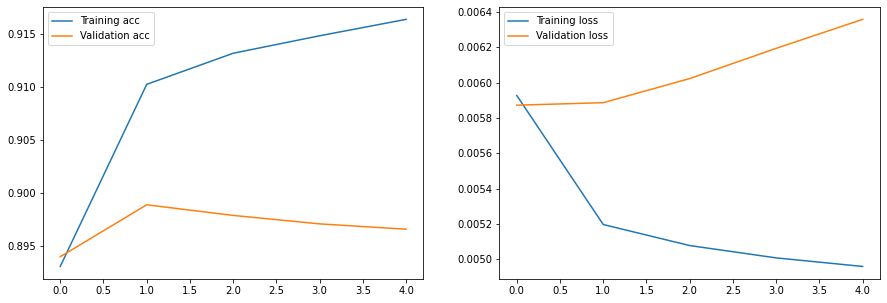
\includegraphics[width=0.9\linewidth,keepaspectratio]{pyt45}
\end{center}

The diagram on the left shows the training accuracy increasing (which corresponds to the network learning to classify our training data better and better), while validation accuracy starts to fall. The diagram on the right show the training loss and validation loss, you can see the training loss decreasing (meaning its performing better) and the validation loss increasing (meaning its performing worse). These graphs would indicate the model is overfitted.

\tiny{(Ref: Microsoft - Intro to Machine Learning using Pytorch)}
\end{frame}

%%%%%%%%%%%%%%%%%%%%%%%%%%%%%%%%%%%%%%%%%%%%%%%%%%%
\begin{frame}[fragile] \frametitle{Visualizing network weights}

Let's create a \lstinline|weight_tensor| which will have a dimension of $784x10$. This tensor can be obtained by calling the \lstinline|net.parameters()| method. In this example, if we want to see if our number is 0 or not, we will multiply input digit by \lstinline|weight_tensor[0]| and pass the result through a softmax normalization to get the answer. This results in the weight tensor elements somewhat resembling the average shape of the digit it classifies:


\begin{center}
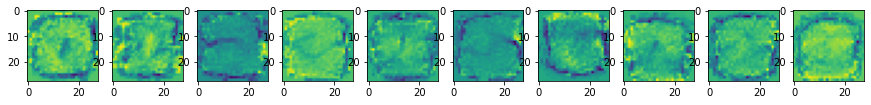
\includegraphics[width=0.9\linewidth,keepaspectratio]{pyt46}
\end{center}


\tiny{(Ref: Microsoft - Intro to Machine Learning using Pytorch)}
\end{frame}


% %%%%%%%%%%%%%%%%%%%%%%%%%%%%%%%%%%%%%%%%%%%%%%%%%%%
% \begin{frame}[fragile] \frametitle{CNN}
% \begin{center}
% \includegraphics[width=0.8\linewidth,keepaspectratio]{pyhun42}
% \end{center}
% First few layers are convoution+subsampling and at the end dense
% \end{frame}


% %%%%%%%%%%%%%%%%%%%%%%%%%%%%%%%%%%%%%%%%%%%%%%%%%%%
% \begin{frame}[fragile] \frametitle{Convolution}
% \begin{center}
% \includegraphics[width=0.8\linewidth,keepaspectratio]{pyhun43}
% \end{center}
% Looking at small portion of image, generating feature maps, one for each filter.
% \end{frame}

% %%%%%%%%%%%%%%%%%%%%%%%%%%%%%%%%%%%%%%%%%%%%%%%%%%%
% \begin{frame}[fragile] \frametitle{Convolution}
% \begin{center}
% \includegraphics[width=0.8\linewidth,keepaspectratio]{pyhun44}
% \end{center}
% First layer had 6 filters and the second has 10.
% \end{frame}


% %%%%%%%%%%%%%%%%%%%%%%%%%%%%%%%%%%%%%%%%%%%%%%%%%%%
% \begin{frame}[fragile] \frametitle{Pooling/Sub-sampling}
% \begin{center}
% \includegraphics[width=0.8\linewidth,keepaspectratio]{pyhun45}
% \end{center}

% \end{frame}


% %%%%%%%%%%%%%%%%%%%%%%%%%%%%%%%%%%%%%%%%%%%%%%%%%%%
% \begin{frame}[fragile] \frametitle{Difference}
% \begin{center}
% \includegraphics[width=0.8\linewidth,keepaspectratio]{pyhun46}
% \end{center}
% CNN is more flexible as it looks are smaller data, so smaller weights.
% \end{frame}


% %%%%%%%%%%%%%%%%%%%%%%%%%%%%%%%%%%%%%%%%%%%%%%%%%%%
% \begin{frame}[fragile] \frametitle{Simple CNN for MNIST}
% \begin{center}
% \includegraphics[width=0.8\linewidth,keepaspectratio]{pyhun47}
% \end{center}
% Using ready Conv2d layer with 1 input channel (greyscale), output channel = 10 (labels).
% \end{frame}


% %%%%%%%%%%%%%%%%%%%%%%%%%%%%%%%%%%%%%%%%%%%%%%%%%%%
% \begin{frame}[fragile] \frametitle{Simple CNN for MNIST}
% \begin{center}
% \includegraphics[width=0.8\linewidth,keepaspectratio]{pyhun48}
% \end{center}

% Outputs and Inputs need to be adjusted properly.  Calculating size after second pooling is not trivial, so just put some value and run. You will get error, suggesting a correct value. 64 is batch size, 320 is the flattened vector. Put 320 there.
% \end{frame}

% %%%%%%%%%%%%%%%%%%%%%%%%%%%%%%%%%%%%%%%%%%%%%%%%%%%
% \begin{frame}[fragile] \frametitle{Simple CNN for MNIST}
% \begin{center}
% \includegraphics[width=\linewidth,keepaspectratio]{pyhun49}
% \end{center}


% \end{frame}






% %%%%%%%%%%%%%%%%%%%%%%%%%%%%%%%%%%%%%%%%%%%%%%%%%%%
% \begin{frame}
  % \begin{center}
    % {\Large CNN using PyTorch: Comprehensive}
    
% \tiny{(Ref: Pytorch Official documentation + few other sources, like Lyman Lin (NTU)))}
  % \end{center}
% \end{frame}



% %%%%%%%%%%%%%%%%%%%%%%%%%%%%%%%%%%%%%%%%%%%%%%%%%%%
% \begin{frame}[fragile] \frametitle{How CNN Works}
% \begin{center}
% \includegraphics[width=0.8\linewidth,keepaspectratio]{pyt20}
% \end{center}

% \end{frame}

% %%%%%%%%%%%%%%%%%%%%%%%%%%%%%%%%%%%%%%%%%%%%%%%%%%%
% \begin{frame}[fragile] \frametitle{How CNN Works}
% \begin{center}
% \includegraphics[width=0.8\linewidth,keepaspectratio]{pyt21}
% \end{center}

% \end{frame}

% %%%%%%%%%%%%%%%%%%%%%%%%%%%%%%%%%%%%%%%%%%%%%%%%%%%
% \begin{frame}[fragile] \frametitle{How CNN Works}
% \begin{center}
% \includegraphics[width=0.8\linewidth,keepaspectratio]{pyt22}
% \end{center}

% \end{frame}

% %%%%%%%%%%%%%%%%%%%%%%%%%%%%%%%%%%%%%%%%%%%%%%%%%%%
% \begin{frame}[fragile] \frametitle{How CNN Works}
% \begin{center}
% \includegraphics[width=0.8\linewidth,keepaspectratio]{pyt23}
% \end{center}

% \end{frame}

% %%%%%%%%%%%%%%%%%%%%%%%%%%%%%%%%%%%%%%%%%%%%%%%%%%%
% \begin{frame}[fragile] \frametitle{How CNN Works}
% \begin{center}
% \includegraphics[width=0.8\linewidth,keepaspectratio]{pyt24}
% \end{center}

% \end{frame}

% %%%%%%%%%%%%%%%%%%%%%%%%%%%%%%%%%%%%%%%%%%%%%%%%%%%
% \begin{frame}[fragile] \frametitle{How CNN Works}
% \begin{center}
% \includegraphics[width=0.8\linewidth,keepaspectratio]{pyt25}
% \end{center}

% \end{frame}

% %%%%%%%%%%%%%%%%%%%%%%%%%%%%%%%%%%%%%%%%%%%%%%%%%%%
% \begin{frame}[fragile] \frametitle{How CNN Works}
% \begin{center}
% \includegraphics[width=0.8\linewidth,keepaspectratio]{pyt26}
% \end{center}

% \end{frame}

% %%%%%%%%%%%%%%%%%%%%%%%%%%%%%%%%%%%%%%%%%%%%%%%%%%%
% \begin{frame}[fragile] \frametitle{How CNN Works}
% \begin{center}
% \includegraphics[width=0.8\linewidth,keepaspectratio]{pyt27}
% \end{center}

% \end{frame}


% %%%%%%%%%%%%%%%%%%%%%%%%%%%%%%%%%%%%%%%%%%%%%%%%%%%
% \begin{frame}[fragile] \frametitle{How CNN Works}
% \begin{center}
% \includegraphics[width=0.8\linewidth,keepaspectratio]{pyt28}
% \end{center}

% \end{frame}
% %%%%%%%%%%%%%%%%%%%%%%%%%%%%%%%%%%%%%%%%%%%%%%%%%%%
% \begin{frame}[fragile] \frametitle{How CNN Works}
% \begin{center}
% \includegraphics[width=0.8\linewidth,keepaspectratio]{pyt29}
% \end{center}

% \end{frame}


% %%%%%%%%%%%%%%%%%%%%%%%%%%%%%%%%%%%%%%%%%%%%%%%%%%%
% \begin{frame}[fragile] \frametitle{How CNN Works}
% \begin{center}
% \includegraphics[width=0.8\linewidth,keepaspectratio]{pyt6}
% \end{center}

% \end{frame}

% %%%%%%%%%%%%%%%%%%%%%%%%%%%%%%%%%%%%%%%%%%%%%%%%%%%
% \begin{frame}[fragile] \frametitle{How CNN Works}
% \begin{center}
% \includegraphics[width=0.8\linewidth,keepaspectratio]{pyt7}
% \end{center}

% \end{frame}


% %%%%%%%%%%%%%%%%%%%%%%%%%%%%%%%%%%%%%%%%%%%%%%%%%%%
% \begin{frame}[fragile] \frametitle{Define the network}
% \begin{lstlisting}
% import torch
% from torch.autograd import Variable
% import torch.nn as nn
% import torch.nn.functional as F

% class Net(nn.Module):
	% pass
	
% net = Net()
% print(net)
% \end{lstlisting}
% \end{frame}

% %%%%%%%%%%%%%%%%%%%%%%%%%%%%%%%%%%%%%%%%%%%%%%%%%%%
% \begin{frame}[fragile] \frametitle{Define the network}
% \begin{lstlisting}
% class Net(nn.Module):

    % def __init__(self):
        % super(Net, self).__init__()
        % # 1 input image channel, 6 output channels, 5x5 square convolution
        % # kernel
        % self.conv1 = nn.Conv2d(1, 6, 5)
        % self.conv2 = nn.Conv2d(6, 16, 5)
        % # an affine operation: y = Wx + b
        % self.fc1 = nn.Linear(16 * 5 * 5, 120)
        % self.fc2 = nn.Linear(120, 84)
        % self.fc3 = nn.Linear(84, 10)
% \end{lstlisting}
% \end{frame}



% %%%%%%%%%%%%%%%%%%%%%%%%%%%%%%%%%%%%%%%%%%%%%%%%%%%
% \begin{frame}[fragile] \frametitle{Define the network}
% \begin{lstlisting}
% class Net(nn.Module):

    % def forward(self, x):
        % # Max pooling over a (2, 2) window
        % x = F.max_pool2d(F.relu(self.conv1(x)), (2, 2))
        % # If the size is a square you can only specify a single number
        % x = F.max_pool2d(F.relu(self.conv2(x)), 2)
        % x = x.view(-1, self.num_flat_features(x))
        % x = F.relu(self.fc1(x))
        % x = F.relu(self.fc2(x))
        % x = self.fc3(x)
        % return x
% \end{lstlisting}
% \end{frame}

% %%%%%%%%%%%%%%%%%%%%%%%%%%%%%%%%%%%%%%%%%%%%%%%%%%%
% \begin{frame}[fragile] \frametitle{How CNN Works}
% \begin{center}
% \includegraphics[width=0.8\linewidth,keepaspectratio]{pyt8}
% \end{center}

% \end{frame}

% %%%%%%%%%%%%%%%%%%%%%%%%%%%%%%%%%%%%%%%%%%%%%%%%%%%
% \begin{frame}[fragile] \frametitle{How CNN Works}
% \begin{center}
% \includegraphics[width=0.8\linewidth,keepaspectratio]{pyt9}
% \end{center}

% \end{frame}

% %%%%%%%%%%%%%%%%%%%%%%%%%%%%%%%%%%%%%%%%%%%%%%%%%%%
% \begin{frame}[fragile] \frametitle{How CNN Works}
% \begin{center}
% \includegraphics[width=0.8\linewidth,keepaspectratio]{pyt10}
% \end{center}

% \end{frame}

% %%%%%%%%%%%%%%%%%%%%%%%%%%%%%%%%%%%%%%%%%%%%%%%%%%%
% \begin{frame}[fragile] \frametitle{How CNN Works}
% \begin{center}
% \includegraphics[width=0.8\linewidth,keepaspectratio]{pyt11}
% \end{center}

% \end{frame}

% %%%%%%%%%%%%%%%%%%%%%%%%%%%%%%%%%%%%%%%%%%%%%%%%%%%
% \begin{frame}[fragile] \frametitle{How CNN Works}
% \begin{center}
% \includegraphics[width=0.8\linewidth,keepaspectratio]{pyt12}
% \end{center}

% \end{frame}

% %%%%%%%%%%%%%%%%%%%%%%%%%%%%%%%%%%%%%%%%%%%%%%%%%%%
% \begin{frame}[fragile] \frametitle{How CNN Works}
% \begin{center}
% \includegraphics[width=0.8\linewidth,keepaspectratio]{pyt13}
% \end{center}

% \end{frame}

% %%%%%%%%%%%%%%%%%%%%%%%%%%%%%%%%%%%%%%%%%%%%%%%%%%%
% \begin{frame}[fragile] \frametitle{How CNN Works}
% \begin{center}
% \includegraphics[width=0.8\linewidth,keepaspectratio]{pyt14}
% \end{center}

% \end{frame}

% %%%%%%%%%%%%%%%%%%%%%%%%%%%%%%%%%%%%%%%%%%%%%%%%%%%
% \begin{frame}[fragile] \frametitle{How CNN Works}
% \begin{center}
% \includegraphics[width=0.8\linewidth,keepaspectratio]{pyt15}
% \end{center}

% \end{frame}

% %%%%%%%%%%%%%%%%%%%%%%%%%%%%%%%%%%%%%%%%%%%%%%%%%%%
% \begin{frame}[fragile] \frametitle{How CNN Works}
% \begin{center}
% \includegraphics[width=0.8\linewidth,keepaspectratio]{pyt16}
% \end{center}

% \end{frame}

% %%%%%%%%%%%%%%%%%%%%%%%%%%%%%%%%%%%%%%%%%%%%%%%%%%%
% \begin{frame}[fragile] \frametitle{How CNN Works}
% \begin{center}
% \includegraphics[width=0.8\linewidth,keepaspectratio]{pyt17}
% \end{center}

% \end{frame}

% %%%%%%%%%%%%%%%%%%%%%%%%%%%%%%%%%%%%%%%%%%%%%%%%%%%
% \begin{frame}[fragile] \frametitle{How CNN Works}
% \begin{center}
% \includegraphics[width=0.8\linewidth,keepaspectratio]{pyt18}
% \end{center}

% \end{frame}

% %%%%%%%%%%%%%%%%%%%%%%%%%%%%%%%%%%%%%%%%%%%%%%%%%%%
% \begin{frame}[fragile] \frametitle{How CNN Works}
% \begin{center}
% \includegraphics[width=0.8\linewidth,keepaspectratio]{pyt19}
% \end{center}
% \tiny{(Reference:PyTorch Tutorial-NTU Machine Learning Course-Lyman Lin )}
% \end{frame}
